\ylDisplay{Silm} % Ülesande nimi
{Tundmatu autor} % Autor
{piirkonnavoor} % Voor
{2004} % Aasta
{P 3} % Ülesande nr.
{1} % Raskustase
{
% Teema: Valgusõpetus
\ifStatement
Tasapeegel asub laual. Vaatame tasapeeglisse ja suleme ühe silma. Asetame peeglile 10-sendilise mundi nii, et see kataks suletud silma kujutise. Avame nüüd pead liigutamata suletud silma ja suleme teise silma. Kus asub nüüd münt näo kujutise suhtes? Põhjendage nähtut. Vahendid: tasapeegel, 10-sendine münt.
\fi

\ifHint
Ülesande lihtsamaks lahendamiseks tuleb konstrueerida joonis ning lahendada probleem läbi tekkivate sarnaste kolmnurkade.
\fi


\ifSolution
Näeme, et 10-sendiline asub jälle suletud silma kujutise kohal. Suletud silma $B$ kujutis tekib peegli taha punkti $B_1 (BO = OB_1)$. Seda me näeme ühe lahtise silmaga $A$ ja katame nähtava kujutise 10-sendilisega kinni punktis $O_1$. Kolmnurgad $B_1OO_1$ ja $B_1BA$ on sarnased (kõik nurgad on vastavalt võrdsed). Kuna $B_1O = \frac{B_1B}{2}$, siis ka $O_1O = \frac{AB}{2}$. 
\begin{center}
	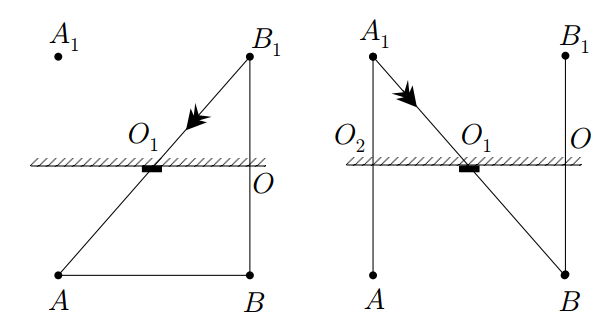
\includegraphics[width=0.5\linewidth]{2004-v2p-03-lah.PNG}
\end{center}
Kui suleme teise silma ($A$), siis punktis $O_1$ olev 10-sendiline katab jälle suletud silma kujutise ($A_1$), sest $OO_1 = O_1O_2$.
\fi
}